% Options for packages loaded elsewhere
\PassOptionsToPackage{unicode}{hyperref}
\PassOptionsToPackage{hyphens}{url}
\PassOptionsToPackage{dvipsnames,svgnames,x11names}{xcolor}
%
\documentclass[
  letterpaper,
  DIV=11,
  numbers=noendperiod]{scrreprt}

\usepackage{amsmath,amssymb}
\usepackage{iftex}
\ifPDFTeX
  \usepackage[T1]{fontenc}
  \usepackage[utf8]{inputenc}
  \usepackage{textcomp} % provide euro and other symbols
\else % if luatex or xetex
  \usepackage{unicode-math}
  \defaultfontfeatures{Scale=MatchLowercase}
  \defaultfontfeatures[\rmfamily]{Ligatures=TeX,Scale=1}
\fi
\usepackage{lmodern}
\ifPDFTeX\else  
    % xetex/luatex font selection
\fi
% Use upquote if available, for straight quotes in verbatim environments
\IfFileExists{upquote.sty}{\usepackage{upquote}}{}
\IfFileExists{microtype.sty}{% use microtype if available
  \usepackage[]{microtype}
  \UseMicrotypeSet[protrusion]{basicmath} % disable protrusion for tt fonts
}{}
\makeatletter
\@ifundefined{KOMAClassName}{% if non-KOMA class
  \IfFileExists{parskip.sty}{%
    \usepackage{parskip}
  }{% else
    \setlength{\parindent}{0pt}
    \setlength{\parskip}{6pt plus 2pt minus 1pt}}
}{% if KOMA class
  \KOMAoptions{parskip=half}}
\makeatother
\usepackage{xcolor}
\setlength{\emergencystretch}{3em} % prevent overfull lines
\setcounter{secnumdepth}{5}
% Make \paragraph and \subparagraph free-standing
\ifx\paragraph\undefined\else
  \let\oldparagraph\paragraph
  \renewcommand{\paragraph}[1]{\oldparagraph{#1}\mbox{}}
\fi
\ifx\subparagraph\undefined\else
  \let\oldsubparagraph\subparagraph
  \renewcommand{\subparagraph}[1]{\oldsubparagraph{#1}\mbox{}}
\fi

\usepackage{color}
\usepackage{fancyvrb}
\newcommand{\VerbBar}{|}
\newcommand{\VERB}{\Verb[commandchars=\\\{\}]}
\DefineVerbatimEnvironment{Highlighting}{Verbatim}{commandchars=\\\{\}}
% Add ',fontsize=\small' for more characters per line
\usepackage{framed}
\definecolor{shadecolor}{RGB}{241,243,245}
\newenvironment{Shaded}{\begin{snugshade}}{\end{snugshade}}
\newcommand{\AlertTok}[1]{\textcolor[rgb]{0.68,0.00,0.00}{#1}}
\newcommand{\AnnotationTok}[1]{\textcolor[rgb]{0.37,0.37,0.37}{#1}}
\newcommand{\AttributeTok}[1]{\textcolor[rgb]{0.40,0.45,0.13}{#1}}
\newcommand{\BaseNTok}[1]{\textcolor[rgb]{0.68,0.00,0.00}{#1}}
\newcommand{\BuiltInTok}[1]{\textcolor[rgb]{0.00,0.23,0.31}{#1}}
\newcommand{\CharTok}[1]{\textcolor[rgb]{0.13,0.47,0.30}{#1}}
\newcommand{\CommentTok}[1]{\textcolor[rgb]{0.37,0.37,0.37}{#1}}
\newcommand{\CommentVarTok}[1]{\textcolor[rgb]{0.37,0.37,0.37}{\textit{#1}}}
\newcommand{\ConstantTok}[1]{\textcolor[rgb]{0.56,0.35,0.01}{#1}}
\newcommand{\ControlFlowTok}[1]{\textcolor[rgb]{0.00,0.23,0.31}{#1}}
\newcommand{\DataTypeTok}[1]{\textcolor[rgb]{0.68,0.00,0.00}{#1}}
\newcommand{\DecValTok}[1]{\textcolor[rgb]{0.68,0.00,0.00}{#1}}
\newcommand{\DocumentationTok}[1]{\textcolor[rgb]{0.37,0.37,0.37}{\textit{#1}}}
\newcommand{\ErrorTok}[1]{\textcolor[rgb]{0.68,0.00,0.00}{#1}}
\newcommand{\ExtensionTok}[1]{\textcolor[rgb]{0.00,0.23,0.31}{#1}}
\newcommand{\FloatTok}[1]{\textcolor[rgb]{0.68,0.00,0.00}{#1}}
\newcommand{\FunctionTok}[1]{\textcolor[rgb]{0.28,0.35,0.67}{#1}}
\newcommand{\ImportTok}[1]{\textcolor[rgb]{0.00,0.46,0.62}{#1}}
\newcommand{\InformationTok}[1]{\textcolor[rgb]{0.37,0.37,0.37}{#1}}
\newcommand{\KeywordTok}[1]{\textcolor[rgb]{0.00,0.23,0.31}{#1}}
\newcommand{\NormalTok}[1]{\textcolor[rgb]{0.00,0.23,0.31}{#1}}
\newcommand{\OperatorTok}[1]{\textcolor[rgb]{0.37,0.37,0.37}{#1}}
\newcommand{\OtherTok}[1]{\textcolor[rgb]{0.00,0.23,0.31}{#1}}
\newcommand{\PreprocessorTok}[1]{\textcolor[rgb]{0.68,0.00,0.00}{#1}}
\newcommand{\RegionMarkerTok}[1]{\textcolor[rgb]{0.00,0.23,0.31}{#1}}
\newcommand{\SpecialCharTok}[1]{\textcolor[rgb]{0.37,0.37,0.37}{#1}}
\newcommand{\SpecialStringTok}[1]{\textcolor[rgb]{0.13,0.47,0.30}{#1}}
\newcommand{\StringTok}[1]{\textcolor[rgb]{0.13,0.47,0.30}{#1}}
\newcommand{\VariableTok}[1]{\textcolor[rgb]{0.07,0.07,0.07}{#1}}
\newcommand{\VerbatimStringTok}[1]{\textcolor[rgb]{0.13,0.47,0.30}{#1}}
\newcommand{\WarningTok}[1]{\textcolor[rgb]{0.37,0.37,0.37}{\textit{#1}}}

\providecommand{\tightlist}{%
  \setlength{\itemsep}{0pt}\setlength{\parskip}{0pt}}\usepackage{longtable,booktabs,array}
\usepackage{calc} % for calculating minipage widths
% Correct order of tables after \paragraph or \subparagraph
\usepackage{etoolbox}
\makeatletter
\patchcmd\longtable{\par}{\if@noskipsec\mbox{}\fi\par}{}{}
\makeatother
% Allow footnotes in longtable head/foot
\IfFileExists{footnotehyper.sty}{\usepackage{footnotehyper}}{\usepackage{footnote}}
\makesavenoteenv{longtable}
\usepackage{graphicx}
\makeatletter
\def\maxwidth{\ifdim\Gin@nat@width>\linewidth\linewidth\else\Gin@nat@width\fi}
\def\maxheight{\ifdim\Gin@nat@height>\textheight\textheight\else\Gin@nat@height\fi}
\makeatother
% Scale images if necessary, so that they will not overflow the page
% margins by default, and it is still possible to overwrite the defaults
% using explicit options in \includegraphics[width, height, ...]{}
\setkeys{Gin}{width=\maxwidth,height=\maxheight,keepaspectratio}
% Set default figure placement to htbp
\makeatletter
\def\fps@figure{htbp}
\makeatother
% definitions for citeproc citations
\NewDocumentCommand\citeproctext{}{}
\NewDocumentCommand\citeproc{mm}{%
  \begingroup\def\citeproctext{#2}\cite{#1}\endgroup}
\makeatletter
 % allow citations to break across lines
 \let\@cite@ofmt\@firstofone
 % avoid brackets around text for \cite:
 \def\@biblabel#1{}
 \def\@cite#1#2{{#1\if@tempswa , #2\fi}}
\makeatother
\newlength{\cslhangindent}
\setlength{\cslhangindent}{1.5em}
\newlength{\csllabelwidth}
\setlength{\csllabelwidth}{3em}
\newenvironment{CSLReferences}[2] % #1 hanging-indent, #2 entry-spacing
 {\begin{list}{}{%
  \setlength{\itemindent}{0pt}
  \setlength{\leftmargin}{0pt}
  \setlength{\parsep}{0pt}
  % turn on hanging indent if param 1 is 1
  \ifodd #1
   \setlength{\leftmargin}{\cslhangindent}
   \setlength{\itemindent}{-1\cslhangindent}
  \fi
  % set entry spacing
  \setlength{\itemsep}{#2\baselineskip}}}
 {\end{list}}
\usepackage{calc}
\newcommand{\CSLBlock}[1]{\hfill\break\parbox[t]{\linewidth}{\strut\ignorespaces#1\strut}}
\newcommand{\CSLLeftMargin}[1]{\parbox[t]{\csllabelwidth}{\strut#1\strut}}
\newcommand{\CSLRightInline}[1]{\parbox[t]{\linewidth - \csllabelwidth}{\strut#1\strut}}
\newcommand{\CSLIndent}[1]{\hspace{\cslhangindent}#1}

\KOMAoption{captions}{tableheading}
\makeatletter
\@ifpackageloaded{bookmark}{}{\usepackage{bookmark}}
\makeatother
\makeatletter
\@ifpackageloaded{caption}{}{\usepackage{caption}}
\AtBeginDocument{%
\ifdefined\contentsname
  \renewcommand*\contentsname{Table of contents}
\else
  \newcommand\contentsname{Table of contents}
\fi
\ifdefined\listfigurename
  \renewcommand*\listfigurename{List of Figures}
\else
  \newcommand\listfigurename{List of Figures}
\fi
\ifdefined\listtablename
  \renewcommand*\listtablename{List of Tables}
\else
  \newcommand\listtablename{List of Tables}
\fi
\ifdefined\figurename
  \renewcommand*\figurename{Figure}
\else
  \newcommand\figurename{Figure}
\fi
\ifdefined\tablename
  \renewcommand*\tablename{Table}
\else
  \newcommand\tablename{Table}
\fi
}
\@ifpackageloaded{float}{}{\usepackage{float}}
\floatstyle{ruled}
\@ifundefined{c@chapter}{\newfloat{codelisting}{h}{lop}}{\newfloat{codelisting}{h}{lop}[chapter]}
\floatname{codelisting}{Listing}
\newcommand*\listoflistings{\listof{codelisting}{List of Listings}}
\makeatother
\makeatletter
\makeatother
\makeatletter
\@ifpackageloaded{caption}{}{\usepackage{caption}}
\@ifpackageloaded{subcaption}{}{\usepackage{subcaption}}
\makeatother
\ifLuaTeX
  \usepackage{selnolig}  % disable illegal ligatures
\fi
\usepackage{bookmark}

\IfFileExists{xurl.sty}{\usepackage{xurl}}{} % add URL line breaks if available
\urlstyle{same} % disable monospaced font for URLs
\hypersetup{
  pdftitle={Multilevel Visualization},
  pdfauthor={Andrew Grogan-Kaylor},
  colorlinks=true,
  linkcolor={blue},
  filecolor={Maroon},
  citecolor={Blue},
  urlcolor={Blue},
  pdfcreator={LaTeX via pandoc}}

\title{Multilevel Visualization}
\author{Andrew Grogan-Kaylor}
\date{2024-03-24}

\begin{document}
\maketitle

\renewcommand*\contentsname{Table of contents}
{
\hypersetup{linkcolor=}
\setcounter{tocdepth}{2}
\tableofcontents
}
\listoffigures
\listoftables
\bookmarksetup{startatroot}

\chapter{Multilevel Visualization}\label{multilevel-visualization}

\section{Introduction}\label{introduction}

Below, I describe the use of \href{https://www.stata.com/}{Stata}
(StataCorp 2021), \href{https://www.r-project.org/}{R} (R Core Team
2023), and \href{https://www.julialang.org/}{Julia} (Bezanson et al.
2017) to visualize multilevel models.

\section{The Data}\label{sec-data}

The examples use the \texttt{simulated\_multilevel\_data.dta} file from
\href{https://agrogan1.github.io/multilevel-thinking/simulated-multi-country-data.html}{\emph{Multilevel
Thinking}}. Here is a
\href{https://github.com/agrogan1/multilevel-multilingual/raw/main/simulated_multilevel_data.dta}{direct
link} to download the data.

\begin{longtable}[]{@{}
  >{\centering\arraybackslash}p{(\columnwidth - 14\tabcolsep) * \real{0.1250}}
  >{\centering\arraybackslash}p{(\columnwidth - 14\tabcolsep) * \real{0.0750}}
  >{\centering\arraybackslash}p{(\columnwidth - 14\tabcolsep) * \real{0.1125}}
  >{\centering\arraybackslash}p{(\columnwidth - 14\tabcolsep) * \real{0.0750}}
  >{\centering\arraybackslash}p{(\columnwidth - 14\tabcolsep) * \real{0.1000}}
  >{\centering\arraybackslash}p{(\columnwidth - 14\tabcolsep) * \real{0.2750}}
  >{\centering\arraybackslash}p{(\columnwidth - 14\tabcolsep) * \real{0.1125}}
  >{\centering\arraybackslash}p{(\columnwidth - 14\tabcolsep) * \real{0.1250}}@{}}

\caption{\label{tbl-multilingual1}Sample of Simulated Multilevel Data}

\tabularnewline

\toprule\noalign{}
\begin{minipage}[b]{\linewidth}\centering
country
\end{minipage} & \begin{minipage}[b]{\linewidth}\centering
HDI
\end{minipage} & \begin{minipage}[b]{\linewidth}\centering
family
\end{minipage} & \begin{minipage}[b]{\linewidth}\centering
id
\end{minipage} & \begin{minipage}[b]{\linewidth}\centering
group
\end{minipage} & \begin{minipage}[b]{\linewidth}\centering
physical\_punishment
\end{minipage} & \begin{minipage}[b]{\linewidth}\centering
warmth
\end{minipage} & \begin{minipage}[b]{\linewidth}\centering
outcome
\end{minipage} \\
\midrule\noalign{}
\endhead
\bottomrule\noalign{}
\endlastfoot
1 & 69 & 1 & 1.1 & 2 & 2 & 3 & 59.18 \\
1 & 69 & 2 & 1.2 & 2 & 4 & 0 & 61.54 \\
1 & 69 & 3 & 1.3 & 1 & 4 & 4 & 51.87 \\
1 & 69 & 4 & 1.4 & 2 & 0 & 6 & 51.71 \\
1 & 69 & 5 & 1.5 & 2 & 3 & 2 & 55.88 \\
1 & 69 & 6 & 1.6 & 1 & 5 & 3 & 60.78 \\

\end{longtable}

\bookmarksetup{startatroot}

\chapter{Graphs}\label{graphs}

\section{Scatterplots}\label{scatterplots}

\subsection{Stata}

\subsubsection{Get The Data}\label{get-the-data}

\begin{Shaded}
\begin{Highlighting}[]

\KeywordTok{use}\NormalTok{ simulated\_multilevel\_data.dta}
\end{Highlighting}
\end{Shaded}

\subsubsection{Scatterplot}\label{scatterplot}

\begin{Shaded}
\begin{Highlighting}[]
\KeywordTok{twoway} \KeywordTok{scatter}\NormalTok{ outcome warmth, }\CommentTok{///}
  \BaseNTok{xtitle}\NormalTok{(}\StringTok{"warmth"}\NormalTok{) }\BaseNTok{ytitle}\NormalTok{(}\StringTok{"outcome"}\NormalTok{) }\CommentTok{///}
  \BaseNTok{title}\NormalTok{(}\StringTok{"Outcome by Parental Warmth"}\NormalTok{) }

\KeywordTok{quietly} \KeywordTok{graph} \KeywordTok{export} \KeywordTok{scatter}\NormalTok{.png, }\KeywordTok{replace}
\end{Highlighting}
\end{Shaded}

\begin{figure}

\centering{

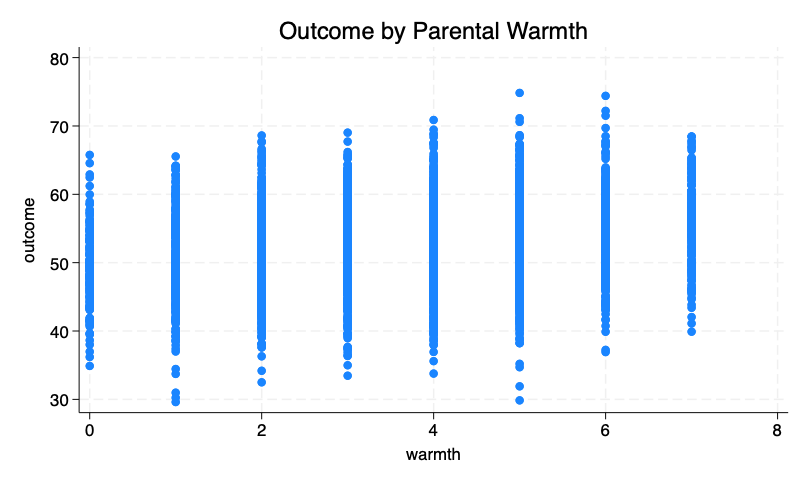
\includegraphics{scatter.png}

}

\caption{\label{fig-Stata}Outcome by Parental Warmth (Stata)}

\end{figure}%

\subsection{R}

\subsubsection{Get The Data}\label{get-the-data-1}

\begin{Shaded}
\begin{Highlighting}[]
\FunctionTok{library}\NormalTok{(haven)}

\NormalTok{df }\OtherTok{\textless{}{-}} \FunctionTok{read\_dta}\NormalTok{(}\StringTok{"simulated\_multilevel\_data.dta"}\NormalTok{)}
\end{Highlighting}
\end{Shaded}

\subsubsection{Scatterplot}\label{scatterplot-1}

\begin{Shaded}
\begin{Highlighting}[]
\FunctionTok{library}\NormalTok{(ggplot2)}

\FunctionTok{ggplot}\NormalTok{(df,}
       \FunctionTok{aes}\NormalTok{(}\AttributeTok{x =}\NormalTok{ warmth,}
           \AttributeTok{y =}\NormalTok{ outcome)) }\SpecialCharTok{+}
  \FunctionTok{geom\_point}\NormalTok{() }\SpecialCharTok{+}
  \FunctionTok{labs}\NormalTok{(}\AttributeTok{title =} \StringTok{"Outcome by Parental Warmth"}\NormalTok{)}
\end{Highlighting}
\end{Shaded}

\begin{figure}[H]

\centering{

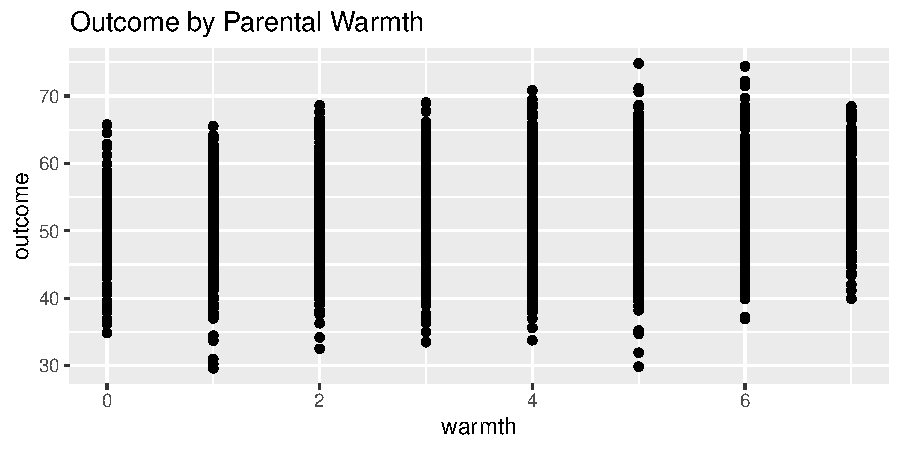
\includegraphics{graphs_files/figure-pdf/fig-R-1.pdf}

}

\caption{\label{fig-R}Outcome by Parental Warmth (R)}

\end{figure}%

\subsection{Julia}

\subsubsection{Get The Data}\label{get-the-data-2}

\begin{Shaded}
\begin{Highlighting}[]
\ImportTok{using} \BuiltInTok{Tables}\NormalTok{, }\BuiltInTok{MixedModels}\NormalTok{, }\BuiltInTok{StatFiles}\NormalTok{, }\BuiltInTok{DataFrames}\NormalTok{, }\BuiltInTok{CategoricalArrays}\NormalTok{, }\BuiltInTok{DataFramesMeta}

\NormalTok{df }\OperatorTok{=} \FunctionTok{DataFrame}\NormalTok{(}\FunctionTok{load}\NormalTok{(}\StringTok{"simulated\_multilevel\_data.dta"}\NormalTok{))}
\end{Highlighting}
\end{Shaded}

\subsubsection{Scatterplot}\label{scatterplot-2}

\begin{Shaded}
\begin{Highlighting}[]
\ImportTok{using} \BuiltInTok{StatsPlots}

\PreprocessorTok{@df}\NormalTok{ df }\FunctionTok{scatter}\NormalTok{(}\OperatorTok{:}\NormalTok{warmth, }\OperatorTok{:}\NormalTok{outcome, }
\NormalTok{               title }\OperatorTok{=} \StringTok{"Outcome by Parental Warmth"}\NormalTok{,}
\NormalTok{               ylabel }\OperatorTok{=} \StringTok{"outcome"}\NormalTok{,}
\NormalTok{               xlabel }\OperatorTok{=} \StringTok{"parental warmth"}\NormalTok{)}
\end{Highlighting}
\end{Shaded}

\begin{figure}[H]

\centering{

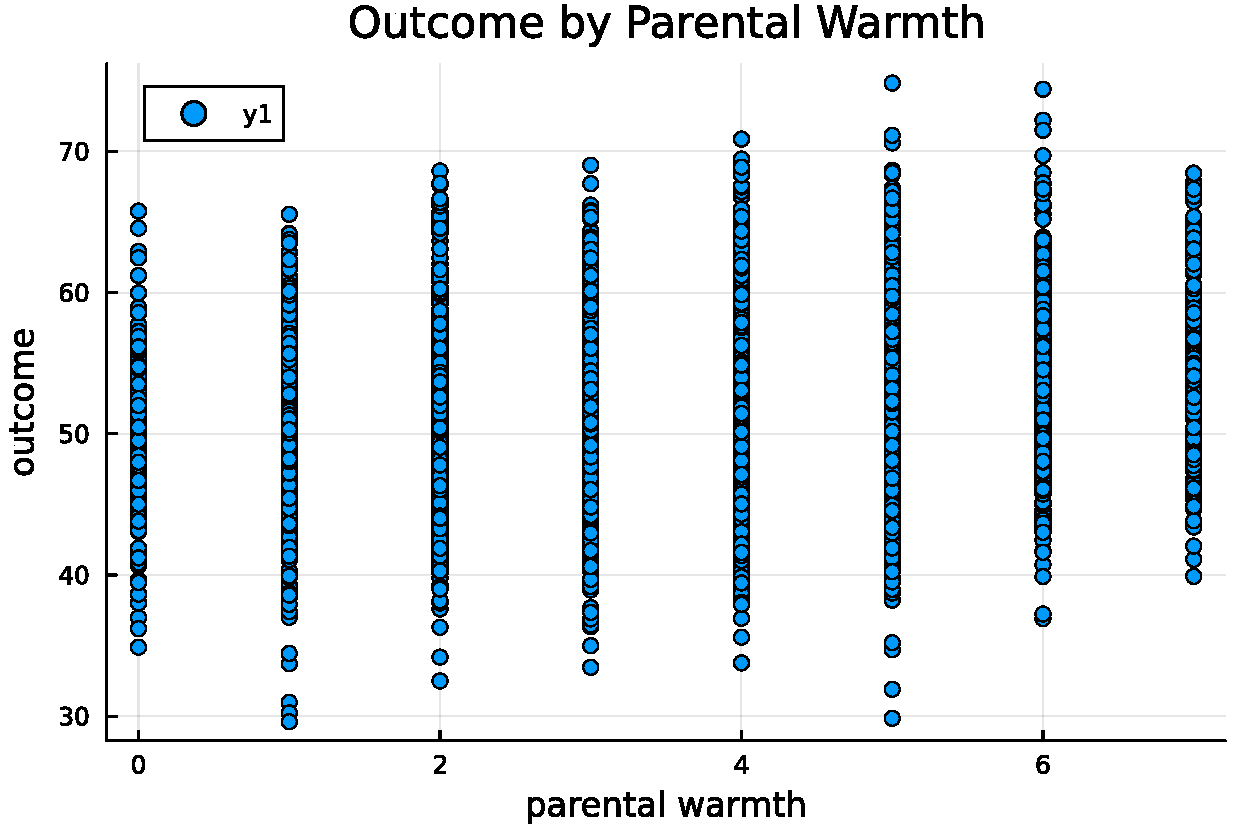
\includegraphics{graphs_files/figure-pdf/fig-Julia-J1.pdf}

}

\caption{\label{fig-Julia}Outcome by Parental Warmth (Julia)}

\end{figure}%

\section{Line Graph}\label{line-graph}

\subsection{Stata}

\subsubsection{Get The Data}\label{get-the-data-3}

\begin{Shaded}
\begin{Highlighting}[]

\KeywordTok{use}\NormalTok{ simulated\_multilevel\_longitudinal\_data.dta}
\end{Highlighting}
\end{Shaded}

\subsubsection{Line Graph}\label{line-graph-1}

\begin{Shaded}
\begin{Highlighting}[]
\KeywordTok{twoway} \KeywordTok{lfit}\NormalTok{ outcome t, }\CommentTok{///}
  \BaseNTok{xtitle}\NormalTok{(}\StringTok{"time"}\NormalTok{) }\BaseNTok{ytitle}\NormalTok{(}\StringTok{"outcome"}\NormalTok{) }\CommentTok{///}
  \BaseNTok{title}\NormalTok{(}\StringTok{"Outcome by Time"}\NormalTok{) }

\KeywordTok{quietly} \KeywordTok{graph} \KeywordTok{export}\NormalTok{ lfitlongitudinal.png, }\KeywordTok{replace}
\end{Highlighting}
\end{Shaded}

\begin{figure}

\centering{

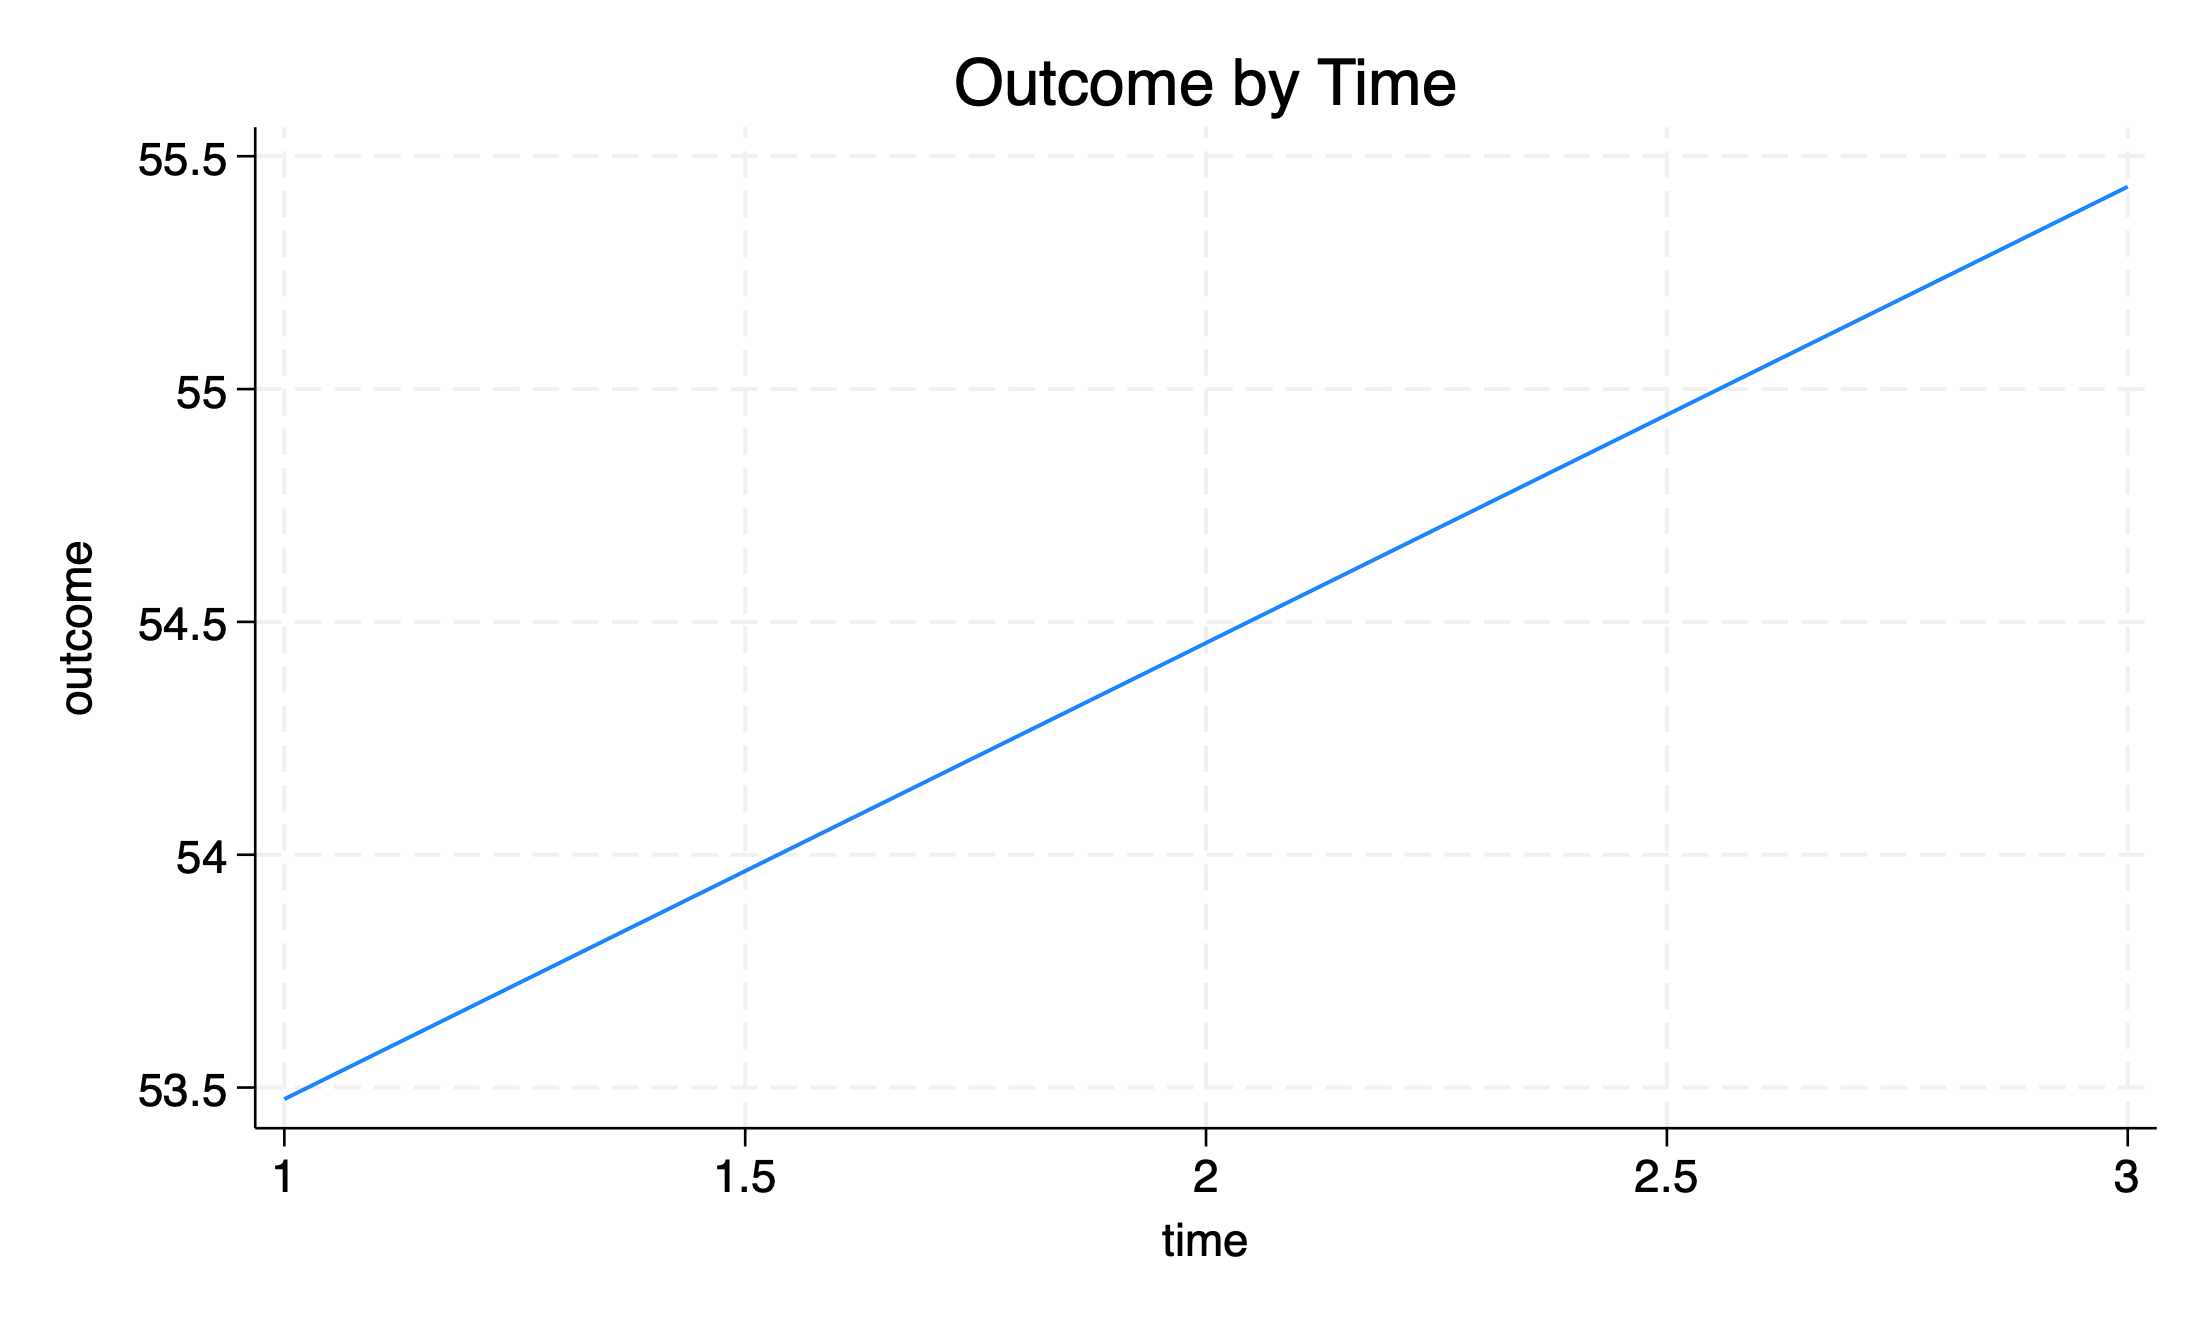
\includegraphics{lfitlongitudinal.png}

}

\caption{\label{fig-Statalongitudinal}Outcome by Parental Warmth
(Stata)}

\end{figure}%

\subsection{R}

\subsubsection{Get The Data}\label{get-the-data-4}

\begin{Shaded}
\begin{Highlighting}[]

\KeywordTok{use}\NormalTok{ simulated\_multilevel\_longitudinal\_data.dta}
\end{Highlighting}
\end{Shaded}

\subsubsection{Line Graph}\label{line-graph-2}

\begin{Shaded}
\begin{Highlighting}[]
\KeywordTok{twoway} \KeywordTok{lfit}\NormalTok{ outcome t, }\CommentTok{///}
  \BaseNTok{xtitle}\NormalTok{(}\StringTok{"time"}\NormalTok{) }\BaseNTok{ytitle}\NormalTok{(}\StringTok{"outcome"}\NormalTok{) }\CommentTok{///}
  \BaseNTok{title}\NormalTok{(}\StringTok{"Outcome by Time"}\NormalTok{) }

\KeywordTok{quietly} \KeywordTok{graph} \KeywordTok{export}\NormalTok{ lfitlongitudinal.png, }\KeywordTok{replace}
\end{Highlighting}
\end{Shaded}

\begin{figure}

\centering{

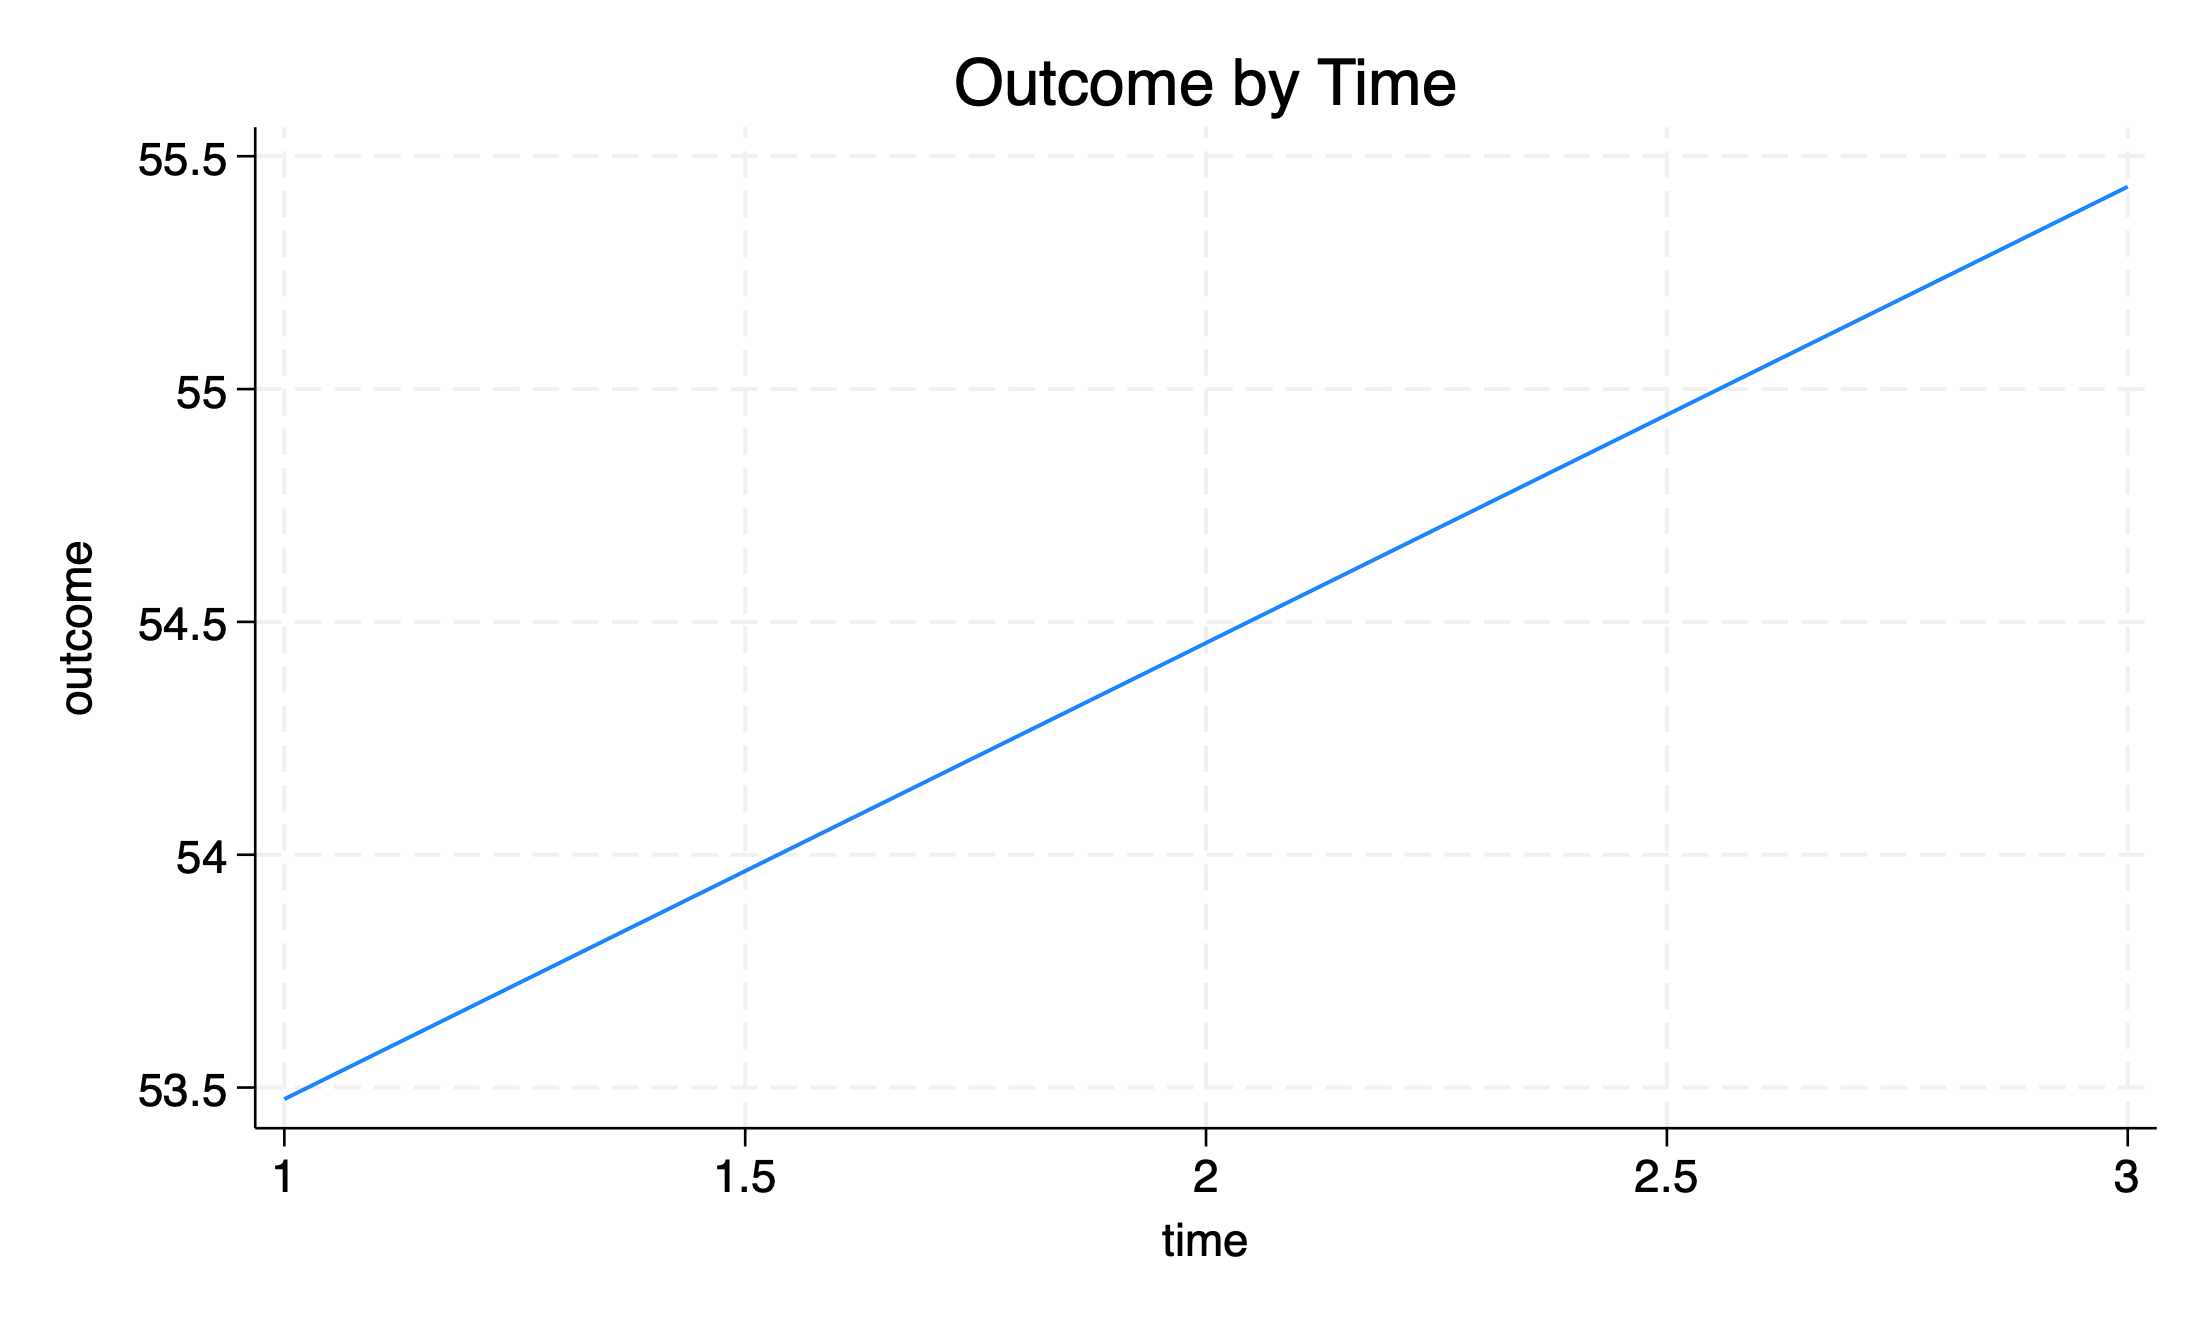
\includegraphics{lfitlongitudinal.png}

}

\caption{\label{fig-Statalongitudinal}Outcome by Parental Warmth
(Stata)}

\end{figure}%

\subsection{Julia}

\subsubsection{Get The Data}\label{get-the-data-5}

\begin{Shaded}
\begin{Highlighting}[]
\ImportTok{using} \BuiltInTok{Tables}\NormalTok{, }\BuiltInTok{MixedModels}\NormalTok{, }\BuiltInTok{StatFiles}\NormalTok{, }\BuiltInTok{DataFrames}\NormalTok{, }\BuiltInTok{CategoricalArrays}\NormalTok{, }\BuiltInTok{DataFramesMeta}

\NormalTok{dfL }\OperatorTok{=} \FunctionTok{DataFrame}\NormalTok{(}\FunctionTok{load}\NormalTok{(}\StringTok{"simulated\_multilevel\_longitudinal\_data.dta"}\NormalTok{))}
\end{Highlighting}
\end{Shaded}

\subsubsection{Line Graph}\label{line-graph-3}

To make our plot with a smoother in Julia, we set the
\texttt{markercolor} and \texttt{markerstrokecolor} to be \emph{white},
and the \texttt{smooth} option to \texttt{:true}.

\begin{Shaded}
\begin{Highlighting}[]
\ImportTok{using} \BuiltInTok{StatsPlots}

\PreprocessorTok{@df}\NormalTok{ dfL }\FunctionTok{scatter}\NormalTok{(}\OperatorTok{:}\NormalTok{t, }\OperatorTok{:}\NormalTok{outcome, }
\NormalTok{               title }\OperatorTok{=} \StringTok{"Outcome by Time"}\NormalTok{,}
\NormalTok{               ylabel }\OperatorTok{=} \StringTok{"outcome"}\NormalTok{,}
\NormalTok{               xlabel }\OperatorTok{=} \StringTok{"time"}\NormalTok{,}
\NormalTok{               markercolor }\OperatorTok{=} \StringTok{"white"}\NormalTok{,}
\NormalTok{               markerstrokecolor }\OperatorTok{=} \StringTok{"white"}\NormalTok{,}
\NormalTok{               smooth}\OperatorTok{=:}\ConstantTok{true}\NormalTok{)}
\end{Highlighting}
\end{Shaded}

\begin{figure}[H]

\centering{

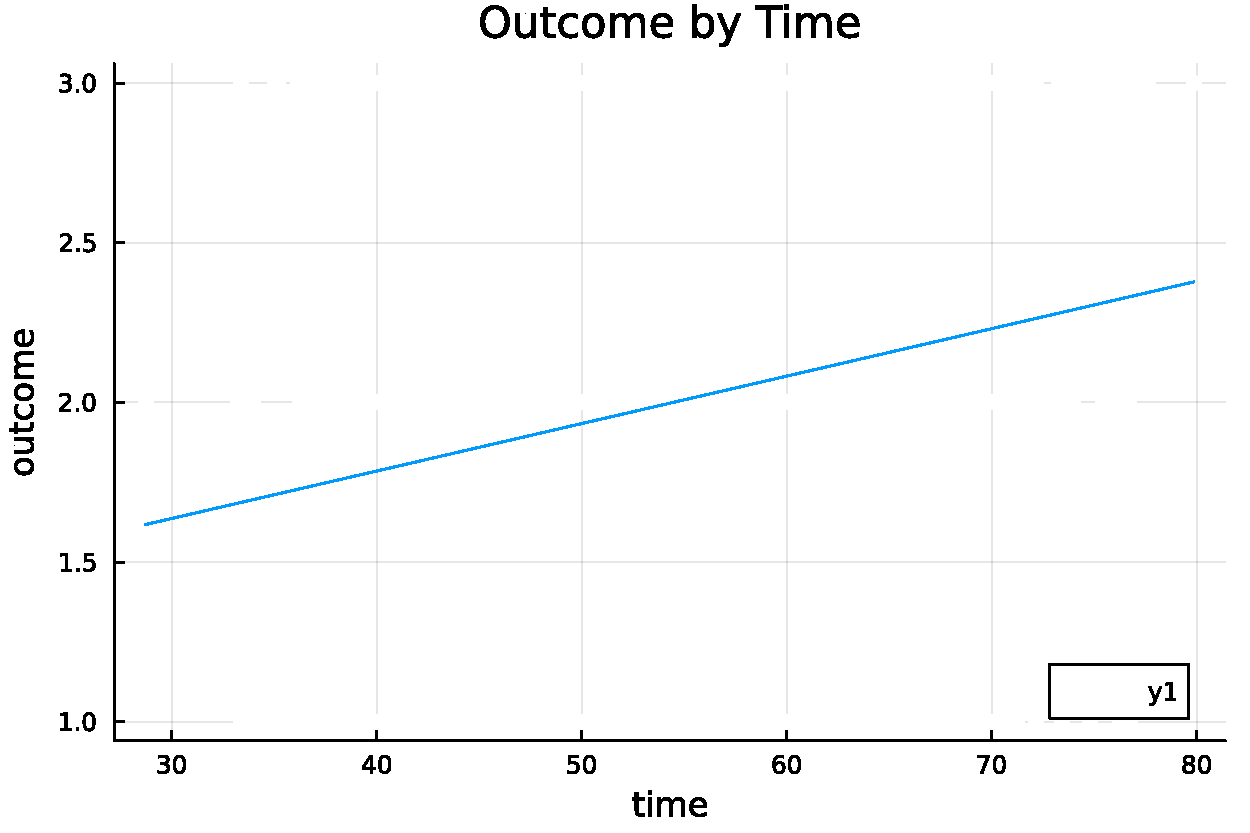
\includegraphics{graphs_files/figure-pdf/fig-Julialongitudinal-J1.pdf}

}

\caption{\label{fig-Julialongitudinal}Outcome by Parental Warmth
(Julia)}

\end{figure}%

\section{Spaghetti Plots}\label{spaghetti-plots}

\subsection{Stata}

\subsection{R}

\subsection{Julia}

\bookmarksetup{startatroot}

\chapter*{References}\label{references}
\addcontentsline{toc}{chapter}{References}

\markboth{References}{References}

\phantomsection\label{refs}
\begin{CSLReferences}{1}{0}
\bibitem[\citeproctext]{ref-JuliaArticle}
Bezanson, Jeff, Alan Edelman, Stefan Karpinski, and Viral B. Shah. 2017.
{``Julia: A Fresh Approach to Numerical Computing.''} \emph{SIAM Review}
59 (1): 65--98. \url{https://doi.org/10.1137/141000671}.

\bibitem[\citeproctext]{ref-RProgram}
R Core Team. 2023. \emph{R: A Language and Environment for Statistical
Computing}. Vienna, Austria: R Foundation for Statistical Computing.
\url{https://www.R-project.org/}.

\bibitem[\citeproctext]{ref-StataCorp2021:3}
StataCorp. 2021. \emph{Stata 17 Graphics Reference Manual}. Stata Press.

\end{CSLReferences}



\end{document}
